% #region PREAMBEL OG PAKKER
\documentclass[a4paper, 12pt]{article}  % DOKUMENTKLASSE
\title{Øving 4}                         % TITTEL
\author{Håvard Solberg Nybøe}           % FORFATTER
\date{MA0001 -- \today}                 % DATO & FAG

\usepackage[english, norsk]{babel}      % NORSK SPRÅK
\usepackage[
    backend=biber,style=apa]{biblatex}  % BIBLIOGRAFI
\usepackage{csquotes}                   % PAKKE TIL BABEL
\addbibresource{bibliografi.bib}        % PATH TIL BIBLIOGRAFI
\usepackage[hidelinks]{hyperref}        % LENKER I TOC OG GENERELT
\usepackage[margin=1in]{geometry}       % VANLIG STØRRELSE MARGIN
\setlength{\parindent}{0em}             % SKILLER AVSNITT
\setlength{\parskip}{.8em}              % SKILLER AVSNITT
\usepackage{graphicx}                   % BILDER \includegraphics[OPTIONS]{PATH}
\usepackage{kantlipsum}                 % FYLLTEKST I KANT-STIL (kant[n-m])
\usepackage{amsfonts,amsmath,amssymb}   % BLACKBOARD BOLD FONT (\mathbb{N}) & SYMBOLER
\usepackage{circuitikz,pgfplots}        % LOGISKE PORTER OG KRETSER & TikZ
\usepackage{float}                      % FLOAT
\usetikzlibrary{shapes.geometric, arrows}% STILER TIL FLYTSKJEMA
\tikzstyle{startstop} = [rectangle, rounded corners, minimum width=3cm, minimum height=1cm, text centered, draw=black, fill=red!30]
\tikzstyle{io} = [trapezium, trapezium left angle=70, trapezium right angle=110, minimum width=3cm, minimum height=1cm, text centered, draw=black, fill=blue!30]
\tikzstyle{prosess} = [rectangle, minimum width=3cm, text width=3cm, minimum height=1cm, text centered, draw=black, fill=orange!30]
\tikzstyle{decision} = [diamond, minimum width=3cm, minimum height=1cm, text centered, draw=black, fill=green!30]
\tikzstyle{arrow} = [thick, ->, > = stealth]
% #endregion
\begin{document}

\maketitle
% \tableofcontents % INNHOLDSFORTEGNELSE

\begin{enumerate}
    \item [\boxed{1}]
          \begin{enumerate}
              \item
                    \begin{flalign*}
                        f(x)   & = \frac{1}{x^2-4}                &&\\
                        D_f(x) & = \mathbb{R}, \quad x \neq \pm 2
                    \end{flalign*}
              \item
                    \begin{flalign*}
                        g(x)   & = \sqrt{9- |x-1|}       &&\\
                        D_g(x) & = \left[ -8, 10 \right] &&\\
                        V_g(x) & = \left[ 0, 3 \right]
                    \end{flalign*}
          \end{enumerate}
    \item [\boxed{2}]
          \begin{flalign*}
              f(x)                            & = \frac{10}{1+x^2}        &&\\
              \lim_{x \to \infty} f(x)        & = 0                       &&\\
              \lim_{x \to -\infty} f(x)       & = 0                       &&\\
              f(x) \mbox{ har } &\mbox{en horisontal asymptote i } x = 0 &&\\
              f(0)                            & = \frac{10}{1 + 0^2} = 10 &&\\
              V_f                             & = \left( 0, 10 \right]
          \end{flalign*}
          \newpage
    \item [\boxed{3}] $$h(x) = \left\{
              \begin{array}{rl}
                  x^2,  & \mbox{hvis } x \geqslant  0 \\
                  -x^2, & \mbox{hvis } x < 0
              \end{array} \right.$$
          \begin{figure}[H]
              \begin{center}
                  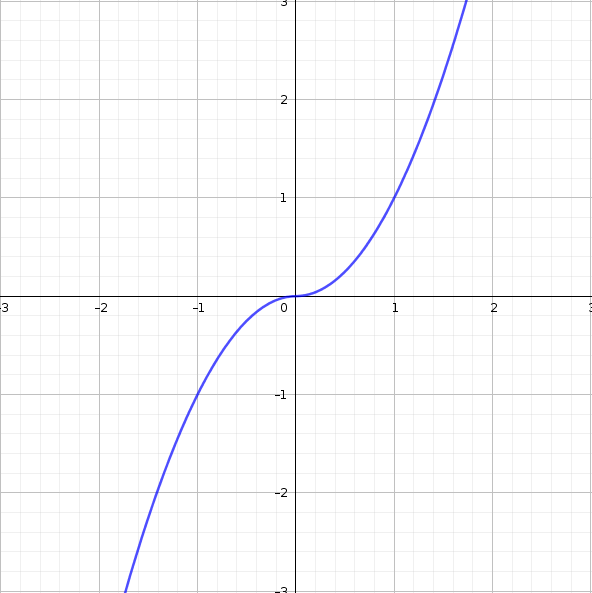
\includegraphics[width=8cm]{graf1.png}
                  \caption{Grafen til $h(x)$}\label{fig:graf1}
              \end{center}
          \end{figure}
          \begin{enumerate}
              \item $V_f = [-\infty, \infty]$
              \item Funksjonen $h(x)$ er injektiv fordi alle verdier av $x$ tilsvarer en unik funksjonsverdi. $\forall a,b \in \mathbb{R} : a \neq b \rightarrow h(a) \neq h(b)$
                    \begin{figure}[H]
                        \begin{center}
                            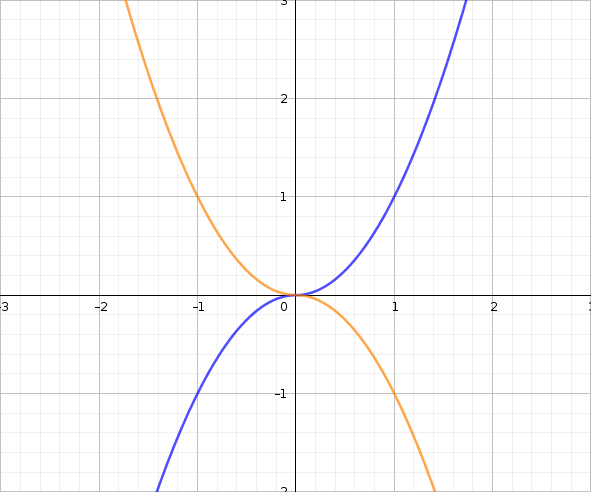
\includegraphics[width=9cm]{Screenshot from 2021-09-26 20-36-05.png}
                            \caption{$h(x)$ og $h^{-1}(x)$}\label{fig:graf2}
                        \end{center}
                    \end{figure}
                    Inversfunksjonen til $h(x)$ er $h^{-1}(x) = \left\{\begin{array}{rl}
                            -x^2, & \mbox{hvis } x \geqslant  0 \\
                            x^2,  & \mbox{hvis } x < 0
                        \end{array}\right.$,
          \end{enumerate}
\end{enumerate}


% \printbibliography[heading=bibintoc] % LAGER BIBLIOGRAFI
\end{document}